
%(BEGIN_QUESTION)
% Copyright 2011, Tony R. Kuphaldt, released under the Creative Commons Attribution License (v 1.0)
% This means you may do almost anything with this work of mine, so long as you give me proper credit

This Allen-Bradley PLC program detects whether an integer number stored in register {\tt N7:4} is odd or even, energizing one of two lights to indicate the result:

$$\includegraphics[width=15.5cm]{i02387x01.eps}$$

Explain how this very simple program detects the oddness or evenness of the integer number, and also determine which output bit activates for the odd result and which activates for the even result.

\vskip 10pt

Could this same programming technique be applied in a Siemens S7-200 PLC, say to determine whether the integer number stored in word {\tt VW88} was odd or even?

\vskip 20pt \vbox{\hrule \hbox{\strut \vrule{} {\bf Suggestions for Socratic discussion} \vrule} \hrule}

\begin{itemize}
\item{} Does the Koyo CLICK PLC offer similar bit-wise addressing capability, which could be used in the same way?
\end{itemize}

\underbar{file i02387}
%(END_QUESTION)





%(BEGIN_ANSWER)

Yes, this same technique may be applied in a Siemens S7-200 PLC.  For a ``word'' (16 bit) integer stored in V memory register {\tt VW88}, the contact bit address would be {\tt V88.0}.
 
%(END_ANSWER)





%(BEGIN_NOTES)

The ``zeroeth'' bit of a binary number is the bit in the 1's place, the only place-weight with an odd value.  Therefore, any odd binary number will have a 1 in this place, while any even binary number will have a 0 in this place.  The status of the least-significant bit (LSB) for any binary number defines its ``oddness'' or ``evenness''.

\vskip 10pt

{\tt O:0/0} is the output activated when {\tt N7:4} is odd (i.e. its LSB is 1).  {\tt O:0/1} is the output activated when {\tt N7:4} is even (i.e. its LSB is 0).  

%INDEX% PLC, ladder logic program analysis and explanation (Allen-Bradley)

%(END_NOTES)


